% Options for packages loaded elsewhere
\PassOptionsToPackage{unicode}{hyperref}
\PassOptionsToPackage{hyphens}{url}
\PassOptionsToPackage{dvipsnames,svgnames*,x11names*}{xcolor}
%
\documentclass[
  ignorenonframetext,
]{beamer}
\usepackage{pgfpages}
\setbeamertemplate{caption}[numbered]
\setbeamertemplate{caption label separator}{: }
\setbeamercolor{caption name}{fg=normal text.fg}
\beamertemplatenavigationsymbolsempty
% Prevent slide breaks in the middle of a paragraph
\widowpenalties 1 10000
\raggedbottom
\setbeamertemplate{part page}{
  \centering
  \begin{beamercolorbox}[sep=16pt,center]{part title}
    \usebeamerfont{part title}\insertpart\par
  \end{beamercolorbox}
}
\setbeamertemplate{section page}{
  \centering
  \begin{beamercolorbox}[sep=12pt,center]{part title}
    \usebeamerfont{section title}\insertsection\par
  \end{beamercolorbox}
}
\setbeamertemplate{subsection page}{
  \centering
  \begin{beamercolorbox}[sep=8pt,center]{part title}
    \usebeamerfont{subsection title}\insertsubsection\par
  \end{beamercolorbox}
}
\AtBeginPart{
  \frame{\partpage}
}
\AtBeginSection{
  \ifbibliography
  \else
    \frame{\sectionpage}
  \fi
}
\AtBeginSubsection{
  \frame{\subsectionpage}
}
\usepackage{lmodern}
\usepackage{amssymb,amsmath}
\usepackage{ifxetex,ifluatex}
\ifnum 0\ifxetex 1\fi\ifluatex 1\fi=0 % if pdftex
  \usepackage[T1]{fontenc}
  \usepackage[utf8]{inputenc}
  \usepackage{textcomp} % provide euro and other symbols
\else % if luatex or xetex
  \usepackage{unicode-math}
  \defaultfontfeatures{Scale=MatchLowercase}
  \defaultfontfeatures[\rmfamily]{Ligatures=TeX,Scale=1}
\fi
% Use upquote if available, for straight quotes in verbatim environments
\IfFileExists{upquote.sty}{\usepackage{upquote}}{}
\IfFileExists{microtype.sty}{% use microtype if available
  \usepackage[]{microtype}
  \UseMicrotypeSet[protrusion]{basicmath} % disable protrusion for tt fonts
}{}
\makeatletter
\@ifundefined{KOMAClassName}{% if non-KOMA class
  \IfFileExists{parskip.sty}{%
    \usepackage{parskip}
  }{% else
    \setlength{\parindent}{0pt}
    \setlength{\parskip}{6pt plus 2pt minus 1pt}}
}{% if KOMA class
  \KOMAoptions{parskip=half}}
\makeatother
\usepackage{xcolor}
\IfFileExists{xurl.sty}{\usepackage{xurl}}{} % add URL line breaks if available
\IfFileExists{bookmark.sty}{\usepackage{bookmark}}{\usepackage{hyperref}}
\hypersetup{
  pdftitle={Classification},
  pdfauthor={Zack Treisman},
  colorlinks=true,
  linkcolor=Maroon,
  filecolor=Maroon,
  citecolor=blue,
  urlcolor=Blue,
  pdfcreator={LaTeX via pandoc}}
\urlstyle{same} % disable monospaced font for URLs
\newif\ifbibliography
\usepackage{color}
\usepackage{fancyvrb}
\newcommand{\VerbBar}{|}
\newcommand{\VERB}{\Verb[commandchars=\\\{\}]}
\DefineVerbatimEnvironment{Highlighting}{Verbatim}{commandchars=\\\{\}}
% Add ',fontsize=\small' for more characters per line
\usepackage{framed}
\definecolor{shadecolor}{RGB}{248,248,248}
\newenvironment{Shaded}{\begin{snugshade}}{\end{snugshade}}
\newcommand{\AlertTok}[1]{\textcolor[rgb]{0.94,0.16,0.16}{#1}}
\newcommand{\AnnotationTok}[1]{\textcolor[rgb]{0.56,0.35,0.01}{\textbf{\textit{#1}}}}
\newcommand{\AttributeTok}[1]{\textcolor[rgb]{0.77,0.63,0.00}{#1}}
\newcommand{\BaseNTok}[1]{\textcolor[rgb]{0.00,0.00,0.81}{#1}}
\newcommand{\BuiltInTok}[1]{#1}
\newcommand{\CharTok}[1]{\textcolor[rgb]{0.31,0.60,0.02}{#1}}
\newcommand{\CommentTok}[1]{\textcolor[rgb]{0.56,0.35,0.01}{\textit{#1}}}
\newcommand{\CommentVarTok}[1]{\textcolor[rgb]{0.56,0.35,0.01}{\textbf{\textit{#1}}}}
\newcommand{\ConstantTok}[1]{\textcolor[rgb]{0.00,0.00,0.00}{#1}}
\newcommand{\ControlFlowTok}[1]{\textcolor[rgb]{0.13,0.29,0.53}{\textbf{#1}}}
\newcommand{\DataTypeTok}[1]{\textcolor[rgb]{0.13,0.29,0.53}{#1}}
\newcommand{\DecValTok}[1]{\textcolor[rgb]{0.00,0.00,0.81}{#1}}
\newcommand{\DocumentationTok}[1]{\textcolor[rgb]{0.56,0.35,0.01}{\textbf{\textit{#1}}}}
\newcommand{\ErrorTok}[1]{\textcolor[rgb]{0.64,0.00,0.00}{\textbf{#1}}}
\newcommand{\ExtensionTok}[1]{#1}
\newcommand{\FloatTok}[1]{\textcolor[rgb]{0.00,0.00,0.81}{#1}}
\newcommand{\FunctionTok}[1]{\textcolor[rgb]{0.00,0.00,0.00}{#1}}
\newcommand{\ImportTok}[1]{#1}
\newcommand{\InformationTok}[1]{\textcolor[rgb]{0.56,0.35,0.01}{\textbf{\textit{#1}}}}
\newcommand{\KeywordTok}[1]{\textcolor[rgb]{0.13,0.29,0.53}{\textbf{#1}}}
\newcommand{\NormalTok}[1]{#1}
\newcommand{\OperatorTok}[1]{\textcolor[rgb]{0.81,0.36,0.00}{\textbf{#1}}}
\newcommand{\OtherTok}[1]{\textcolor[rgb]{0.56,0.35,0.01}{#1}}
\newcommand{\PreprocessorTok}[1]{\textcolor[rgb]{0.56,0.35,0.01}{\textit{#1}}}
\newcommand{\RegionMarkerTok}[1]{#1}
\newcommand{\SpecialCharTok}[1]{\textcolor[rgb]{0.00,0.00,0.00}{#1}}
\newcommand{\SpecialStringTok}[1]{\textcolor[rgb]{0.31,0.60,0.02}{#1}}
\newcommand{\StringTok}[1]{\textcolor[rgb]{0.31,0.60,0.02}{#1}}
\newcommand{\VariableTok}[1]{\textcolor[rgb]{0.00,0.00,0.00}{#1}}
\newcommand{\VerbatimStringTok}[1]{\textcolor[rgb]{0.31,0.60,0.02}{#1}}
\newcommand{\WarningTok}[1]{\textcolor[rgb]{0.56,0.35,0.01}{\textbf{\textit{#1}}}}
\usepackage{graphicx,grffile}
\makeatletter
\def\maxwidth{\ifdim\Gin@nat@width>\linewidth\linewidth\else\Gin@nat@width\fi}
\def\maxheight{\ifdim\Gin@nat@height>\textheight\textheight\else\Gin@nat@height\fi}
\makeatother
% Scale images if necessary, so that they will not overflow the page
% margins by default, and it is still possible to overwrite the defaults
% using explicit options in \includegraphics[width, height, ...]{}
\setkeys{Gin}{width=\maxwidth,height=\maxheight,keepaspectratio}
% Set default figure placement to htbp
\makeatletter
\def\fps@figure{htbp}
\makeatother
\setlength{\emergencystretch}{3em} % prevent overfull lines
\providecommand{\tightlist}{%
  \setlength{\itemsep}{0pt}\setlength{\parskip}{0pt}}
\setcounter{secnumdepth}{-\maxdimen} % remove section numbering

\pgfdeclareimage[width=3.5cm]{mcslogo}{../western_logo_hor_MCS_3C_pos.pdf}
\pgfdeclareimage[width=1cm]{ccbysa}{../ccbysa88x31.png}
\titlegraphic{\href{http://creativecommons.org/licenses/by-sa/4.0/}{\pgfuseimage{ccbysa}}
\hfill
\href{https://western.edu/program/mathematics/}{\pgfuseimage{mcslogo}}}
%\usecolortheme{wcu}
%\institute{Western Colorado University}
%\setbeamertemplate{navigation symbols}{}

\title{Classification}
\author{Zack Treisman}
\date{Spring 2021}

\begin{document}
\frame{\titlepage}

\begin{frame}[fragile]

\begin{Shaded}
\begin{Highlighting}[]
\KeywordTok{library}\NormalTok{(tidyverse)}
\KeywordTok{library}\NormalTok{(caret)}
\KeywordTok{library}\NormalTok{(MASS)}
\KeywordTok{library}\NormalTok{(e1071)}
\KeywordTok{library}\NormalTok{(tree)}
\KeywordTok{library}\NormalTok{(randomForest)}
\KeywordTok{set.seed}\NormalTok{(}\DecValTok{3}\NormalTok{)}
\end{Highlighting}
\end{Shaded}

\end{frame}

\begin{frame}[fragile]{Philosophy}
\protect\hypertarget{philosophy}{}

In all of the modeling we have done so far, the response variable has
been numeric.

\begin{itemize}
\tightlist
\item
  A binomial glm is used when the response is a binary categorical
  variable, but the response in the model is the probability of
  observing the level designated success.
\end{itemize}

What are our options if we wish to predict a categorical response with
more than two levels?

\begin{itemize}
\tightlist
\item
  Nearest-neighbor averaging (KNN, \texttt{class::knn})
\item
  Multinomial logistic regression
\item
  Discriminant analysis (linear, quadratic, naive Bayes, \ldots)
\item
  Classification trees or Random Forests
\item
  Support vector machines, neural networks and other machine learning
  methods
\end{itemize}

\end{frame}

\begin{frame}{Binomial GLMs}
\protect\hypertarget{binomial-glms}{}

Consider a binary categorical variable \(Y\) with classes 0 and 1.

In a binomial GLM, we model the expected probability \(p(x)=P(Y=1|X=x)\)
using \[
\text{logit}(p(x))=\beta_0+\beta_1x_1+\cdots+\beta_mx_m
\] where \[
\text{logit}(p(x))=\log\left(\frac{p(x)}{1-p(x)}\right).
\] Equivalently \[
p(x)=\frac{e^{\beta_0+\beta_1x_1+\cdots+\beta_mx_m}}{1+e^{\beta_0+\beta_1x_1+\cdots+\beta_mx_m}}.
\] When \(Y\) is a categorical variable with more than 2 levels, it
continues to be useful to model the probabilities that it takes each
individual level.

\end{frame}

\begin{frame}[fragile]{Multinomial regression}
\protect\hypertarget{multinomial-regression}{}

This technique seems like it doesn't get used as much. If you are
interested, the tools that do it are \texttt{glmnet::glmnet} with
\texttt{family=multinomial} or \texttt{nnet::multinom}.

\texttt{glmnet} also does Lasso and Ridge Regression, which do something
like dimension reduction by feature selection. See Chapter 6 of James et
al. (2013).

\end{frame}

\begin{frame}{Discriminant Analysis}
\protect\hypertarget{discriminant-analysis}{}

Model the distribution of \(X\) for each class, then apply Bayes'
theorem. We'll follow James et al. (2013) and use the following
notation:

\begin{itemize}
\tightlist
\item
  \(f_k(x)=P(X=x|Y=k)\) is the distribution of \(X\) for class \(k\).
\item
  \(\pi_k=P(Y=k)\) is the prior probability for class \(k\).
\item
  \(p_k(x)=P(Y=k|X=x)\) is the posterior probability for class \(k\).
\end{itemize}

Bayes' theorem says

\[
p_k(x)=\frac{\pi_kf_k(x)}{\sum_{l=1}^{K}\pi_lf_l(x)}.
\] Given \(X=x\), we can choose the class \(k\) for \(Y\) such that
\(p_k(x)\) is largest. Alternatively, we may wish to report all of the
probabilities \(p_k(x)\).

\end{frame}

\begin{frame}{Linear Discriminant Analysis}
\protect\hypertarget{linear-discriminant-analysis}{}

Two strong assumptions make finding the largest \(p_k(x)\) much easier.

\begin{itemize}
\tightlist
\item
  The distributions \(f_k(x)\) are normal.
  \(f_k(x)=\frac{1}{\sigma_k\sqrt{2\pi}}e^{-\frac{1}{2}\left(\frac{x-\mu_k}{\sigma_k}\right)^2}\)
\item
  The variance is the same for all classes: \(\sigma_k=\sigma\).
\end{itemize}

Taking logs of the resulting formulas for \(p_k(x)\) and discarding
terms that don't depend on \(k\) gives the \emph{discriminant}:

\[
\delta_k(x)=x\frac{\mu_k}{\sigma^2} - \frac{\mu_k^2}{2\sigma^2}+\log(\pi_k).
\] This is a linear function of \(x\). It is easy to compute and
\(p_k(x)\) is greatest when \(\delta_k(x)\) is greatest. Find the
\emph{decision boundary} between class \(j\) and class \(k\) by solving
\(\delta_j(x)=\delta_k(x)\).

\begin{itemize}
\tightlist
\item
  The above is written assuming that there is only a single predictor
  \(x\). For multiple predictors, the math is similar, with \(x\)
  replaced by the vector of predictors and \(\sigma\) by the covariance
  matrix. Decision boundaries are linear.
\end{itemize}

\end{frame}

\begin{frame}{LDA illustration}
\protect\hypertarget{lda-illustration}{}

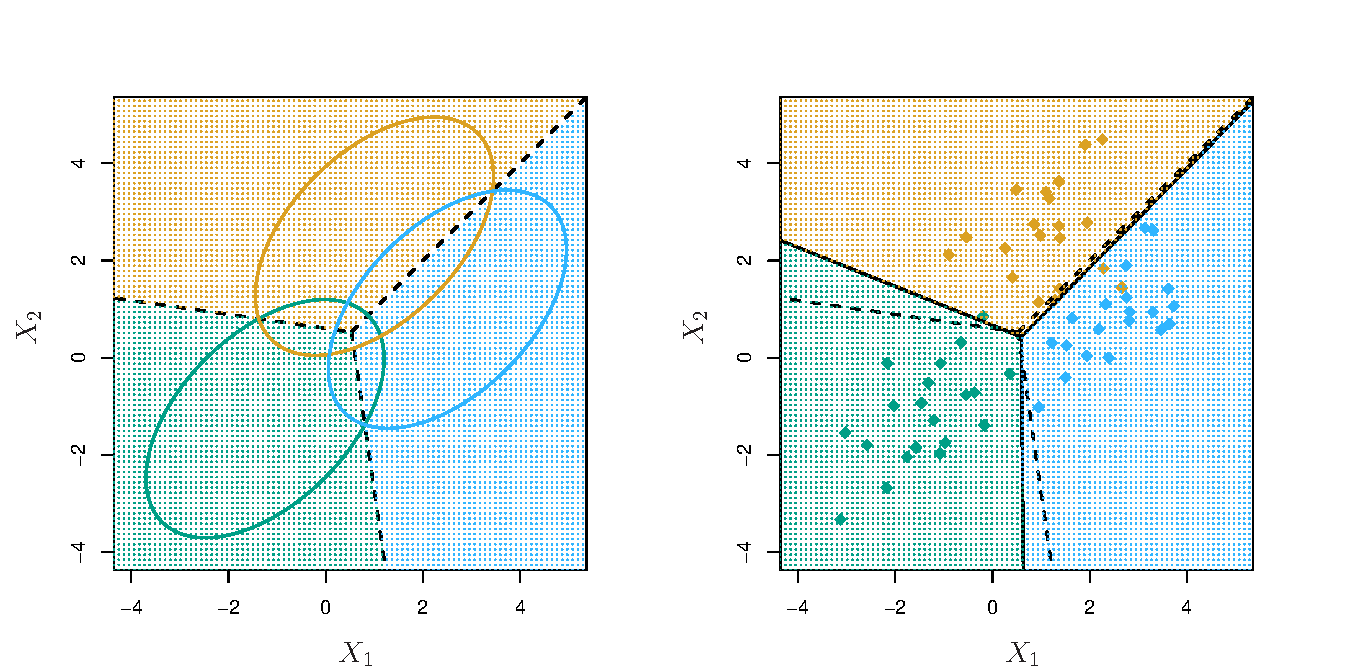
\includegraphics{4.6.pdf}

This graphic is from James et al. (2013). It shows simulated data from
Gaussian distributions indicated by the ovals. Dotted lines are optimal
decision boundaries. Solid lines are decision boundaries from LDA.

\end{frame}

\begin{frame}[fragile]{LDA example}
\protect\hypertarget{lda-example}{}

We'll study Fisher's iris data.

\scriptsize

\begin{Shaded}
\begin{Highlighting}[]
\KeywordTok{pairs}\NormalTok{(iris[,}\DecValTok{1}\OperatorTok{:}\DecValTok{4}\NormalTok{], }\DataTypeTok{col=}\NormalTok{iris}\OperatorTok{$}\NormalTok{Species, }\DataTypeTok{pch=}\DecValTok{19}\NormalTok{)}
\end{Highlighting}
\end{Shaded}

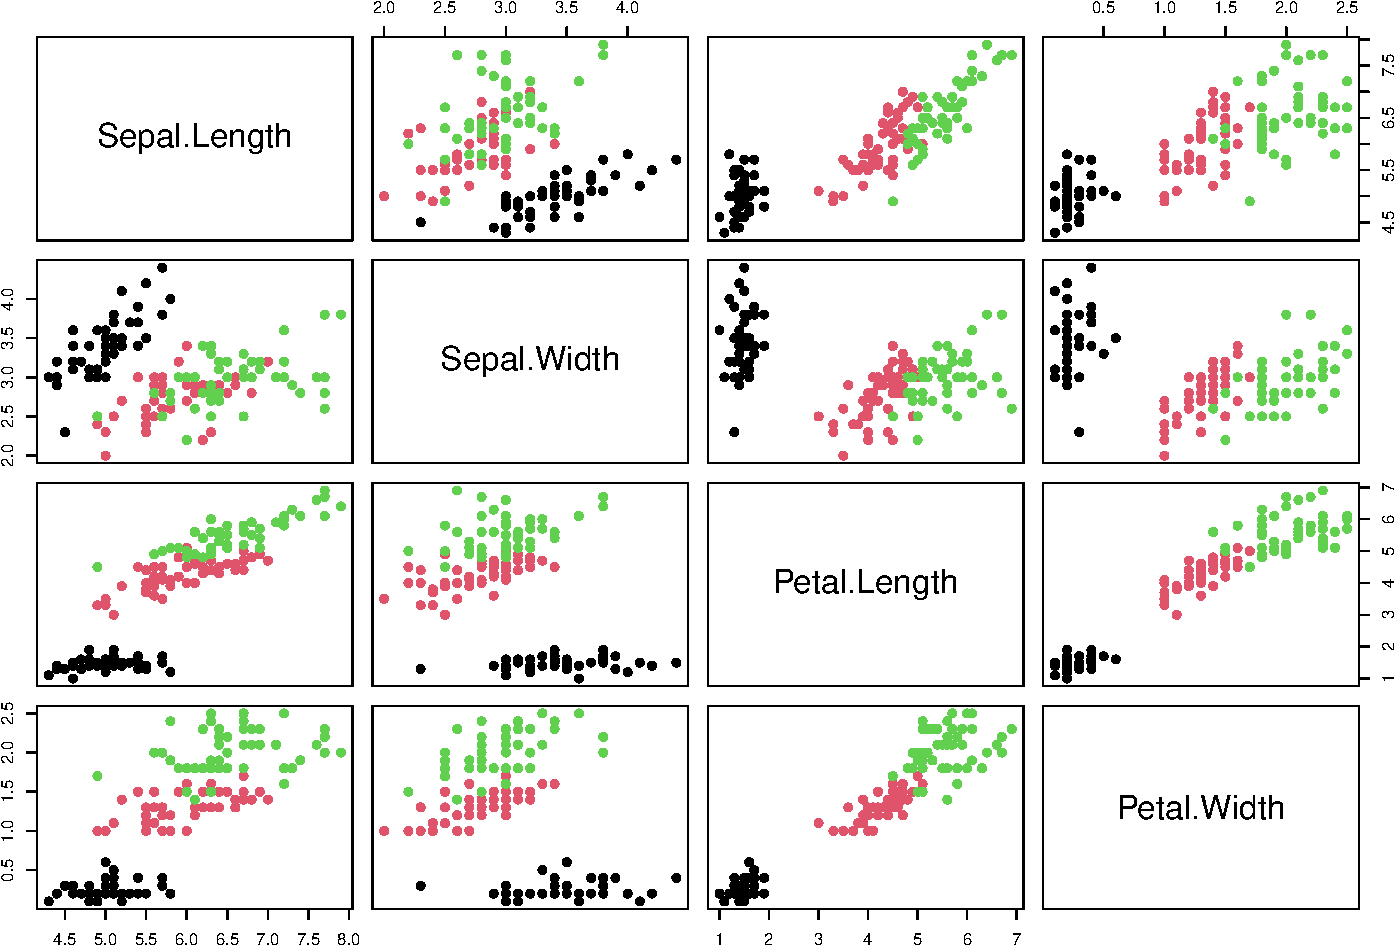
\includegraphics{classify_files/figure-beamer/unnamed-chunk-3-1.pdf}

\end{frame}

\begin{frame}[fragile]{LDA example (model fitting)}
\protect\hypertarget{lda-example-model-fitting}{}

The \texttt{lda} command from \texttt{MASS} performs LDA. The LD1 and
LD2 vectors make a nice basis for the plane spanned by the centroids of
the 3 species.

\tiny

\begin{Shaded}
\begin{Highlighting}[]
\NormalTok{lda.mod <-}\StringTok{ }\KeywordTok{lda}\NormalTok{(Species}\OperatorTok{~}\NormalTok{., }\DataTypeTok{data =}\NormalTok{ iris)}
\NormalTok{lda.mod}
\end{Highlighting}
\end{Shaded}

\begin{verbatim}
## Call:
## lda(Species ~ ., data = iris)
## 
## Prior probabilities of groups:
##     setosa versicolor  virginica 
##  0.3333333  0.3333333  0.3333333 
## 
## Group means:
##            Sepal.Length Sepal.Width Petal.Length Petal.Width
## setosa            5.006       3.428        1.462       0.246
## versicolor        5.936       2.770        4.260       1.326
## virginica         6.588       2.974        5.552       2.026
## 
## Coefficients of linear discriminants:
##                     LD1         LD2
## Sepal.Length  0.8293776  0.02410215
## Sepal.Width   1.5344731  2.16452123
## Petal.Length -2.2012117 -0.93192121
## Petal.Width  -2.8104603  2.83918785
## 
## Proportion of trace:
##    LD1    LD2 
## 0.9912 0.0088
\end{verbatim}

\end{frame}

\begin{frame}[fragile]{LDA example (model evaluation)}
\protect\hypertarget{lda-example-model-evaluation}{}

The model is correct in all but 3 cases. \scriptsize

\begin{Shaded}
\begin{Highlighting}[]
\NormalTok{lda.pred <-}\StringTok{ }\KeywordTok{predict}\NormalTok{(lda.mod)}
\KeywordTok{mean}\NormalTok{(lda.pred}\OperatorTok{$}\NormalTok{class}\OperatorTok{==}\NormalTok{iris}\OperatorTok{$}\NormalTok{Species)}
\end{Highlighting}
\end{Shaded}

\begin{verbatim}
## [1] 0.98
\end{verbatim}

\begin{Shaded}
\begin{Highlighting}[]
\KeywordTok{sum}\NormalTok{(lda.pred}\OperatorTok{$}\NormalTok{class}\OperatorTok{!=}\NormalTok{iris}\OperatorTok{$}\NormalTok{Species)}
\end{Highlighting}
\end{Shaded}

\begin{verbatim}
## [1] 3
\end{verbatim}

\begin{Shaded}
\begin{Highlighting}[]
\NormalTok{lda.obs <-}\StringTok{ }\KeywordTok{as.data.frame}\NormalTok{(lda.pred}\OperatorTok{$}\NormalTok{x)}
\KeywordTok{ggplot}\NormalTok{(lda.obs, }\KeywordTok{aes}\NormalTok{(LD1, LD2, }\DataTypeTok{color=}\NormalTok{lda.pred}\OperatorTok{$}\NormalTok{class))}\OperatorTok{+}\KeywordTok{geom_point}\NormalTok{()}
\end{Highlighting}
\end{Shaded}

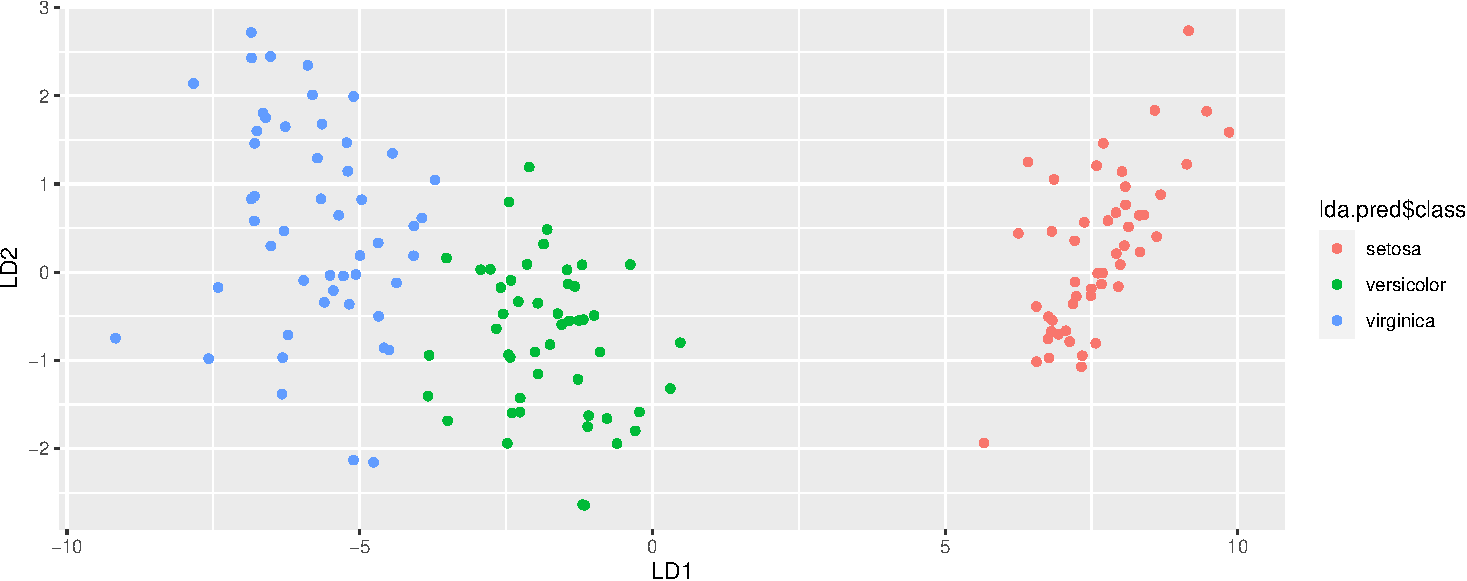
\includegraphics{classify_files/figure-beamer/unnamed-chunk-5-1.pdf}

\end{frame}

\begin{frame}[fragile]{LDA example (posterior probabilities)}
\protect\hypertarget{lda-example-posterior-probabilities}{}

Posterior probabilities are also available from \texttt{predict.lda}.
\scriptsize

\begin{Shaded}
\begin{Highlighting}[]
\NormalTok{lda.post <-}\StringTok{ }\KeywordTok{as.data.frame}\NormalTok{(lda.pred}\OperatorTok{$}\NormalTok{posterior)}
\KeywordTok{ggplot}\NormalTok{(lda.obs, }\KeywordTok{aes}\NormalTok{(LD1, LD2))}\OperatorTok{+}
\StringTok{  }\KeywordTok{geom_point}\NormalTok{(}\KeywordTok{aes}\NormalTok{(}\DataTypeTok{size=}\NormalTok{lda.post}\OperatorTok{$}\NormalTok{setosa, }\DataTypeTok{color=}\StringTok{"setosa"}\NormalTok{), }\DataTypeTok{alpha=}\FloatTok{0.5}\NormalTok{)}\OperatorTok{+}
\StringTok{  }\KeywordTok{geom_point}\NormalTok{(}\KeywordTok{aes}\NormalTok{(}\DataTypeTok{size=}\NormalTok{lda.post}\OperatorTok{$}\NormalTok{virginica, }\DataTypeTok{color=}\StringTok{"virginica"}\NormalTok{), }\DataTypeTok{alpha=}\FloatTok{0.5}\NormalTok{)}\OperatorTok{+}
\StringTok{  }\KeywordTok{geom_point}\NormalTok{(}\KeywordTok{aes}\NormalTok{(}\DataTypeTok{size=}\NormalTok{lda.post}\OperatorTok{$}\NormalTok{versicolor, }\DataTypeTok{color=}\StringTok{"versicolor"}\NormalTok{), }\DataTypeTok{alpha=}\FloatTok{0.5}\NormalTok{)}\OperatorTok{+}
\StringTok{  }\KeywordTok{labs}\NormalTok{(}\DataTypeTok{size=}\StringTok{"Confidence"}\NormalTok{, }\DataTypeTok{color=}\StringTok{"Species"}\NormalTok{)}
\end{Highlighting}
\end{Shaded}

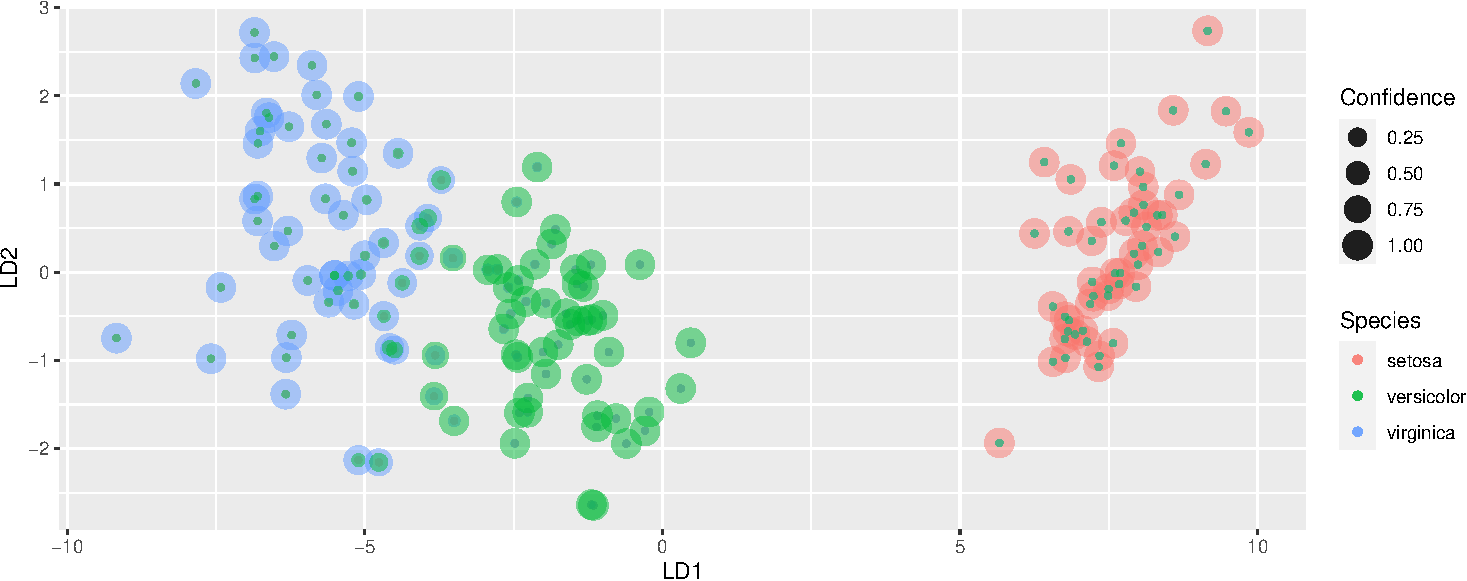
\includegraphics{classify_files/figure-beamer/unnamed-chunk-6-1.pdf}

\end{frame}

\begin{frame}{Quadratic Discriminant Analysis}
\protect\hypertarget{quadratic-discriminant-analysis}{}

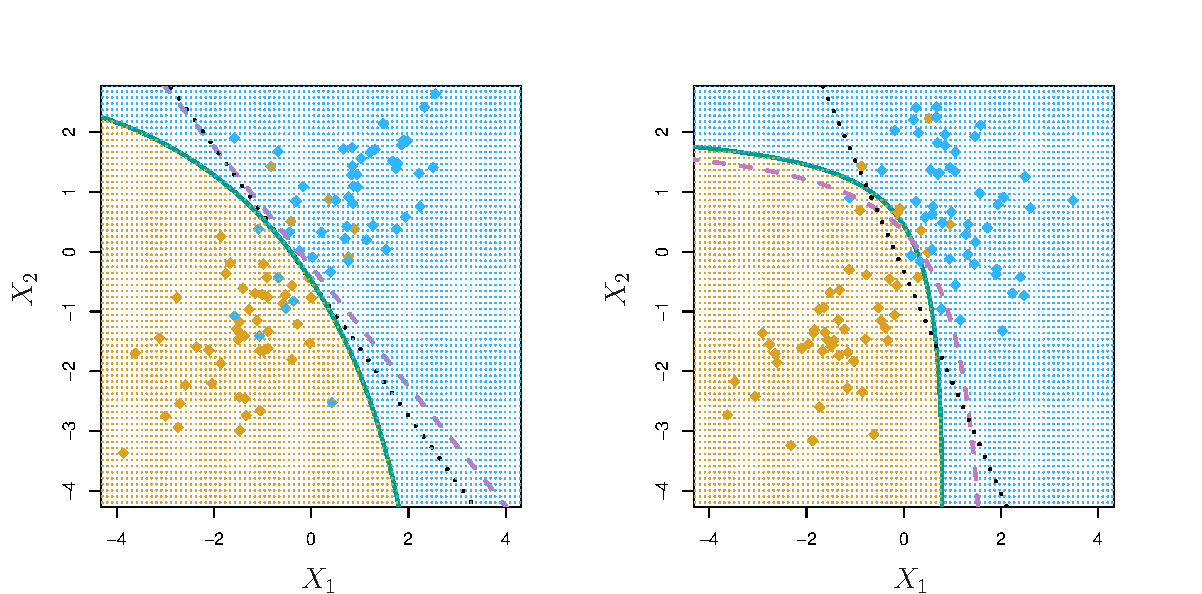
\includegraphics{4.9.pdf}

Keeping the normality assumption but relaxing the condition that all of
the variances are equal leads to \emph{quadratic discriminant analysis}.
The decision boundaries are quadratic instead of linear.

\begin{itemize}
\tightlist
\item
  Smaller data sets do better with LDA.
\end{itemize}

\end{frame}

\begin{frame}[fragile]{QDA example (model fitting)}
\protect\hypertarget{qda-example-model-fitting}{}

QDA doesn't do dimension reduction as a byproduct like LDA.

\scriptsize

\begin{Shaded}
\begin{Highlighting}[]
\NormalTok{qda.mod <-}\StringTok{ }\KeywordTok{qda}\NormalTok{(Species}\OperatorTok{~}\NormalTok{., }\DataTypeTok{data =}\NormalTok{ iris)}
\NormalTok{qda.mod}
\end{Highlighting}
\end{Shaded}

\begin{verbatim}
## Call:
## qda(Species ~ ., data = iris)
## 
## Prior probabilities of groups:
##     setosa versicolor  virginica 
##  0.3333333  0.3333333  0.3333333 
## 
## Group means:
##            Sepal.Length Sepal.Width Petal.Length Petal.Width
## setosa            5.006       3.428        1.462       0.246
## versicolor        5.936       2.770        4.260       1.326
## virginica         6.588       2.974        5.552       2.026
\end{verbatim}

\end{frame}

\begin{frame}[fragile]{QDA example (model evaluation)}
\protect\hypertarget{qda-example-model-evaluation}{}

The predictions from QDA are the same as LDA on these data. \scriptsize

\begin{Shaded}
\begin{Highlighting}[]
\NormalTok{qda.pred <-}\StringTok{ }\KeywordTok{predict}\NormalTok{(qda.mod)}
\KeywordTok{sum}\NormalTok{(qda.pred}\OperatorTok{$}\NormalTok{class}\OperatorTok{!=}\NormalTok{iris}\OperatorTok{$}\NormalTok{Species)}
\end{Highlighting}
\end{Shaded}

\begin{verbatim}
## [1] 3
\end{verbatim}

\begin{Shaded}
\begin{Highlighting}[]
\NormalTok{qda.post <-}\StringTok{ }\KeywordTok{as.data.frame}\NormalTok{(qda.pred}\OperatorTok{$}\NormalTok{posterior)}
\KeywordTok{ggplot}\NormalTok{(lda.obs, }\KeywordTok{aes}\NormalTok{(LD1, LD2))}\OperatorTok{+}
\StringTok{  }\KeywordTok{geom_point}\NormalTok{(}\KeywordTok{aes}\NormalTok{(}\DataTypeTok{size=}\NormalTok{qda.post}\OperatorTok{$}\NormalTok{setosa, }\DataTypeTok{color=}\StringTok{"setosa"}\NormalTok{), }\DataTypeTok{alpha=}\FloatTok{0.5}\NormalTok{)}\OperatorTok{+}
\StringTok{  }\KeywordTok{geom_point}\NormalTok{(}\KeywordTok{aes}\NormalTok{(}\DataTypeTok{size=}\NormalTok{qda.post}\OperatorTok{$}\NormalTok{virginica, }\DataTypeTok{color=}\StringTok{"virginica"}\NormalTok{), }\DataTypeTok{alpha=}\FloatTok{0.5}\NormalTok{)}\OperatorTok{+}
\StringTok{  }\KeywordTok{geom_point}\NormalTok{(}\KeywordTok{aes}\NormalTok{(}\DataTypeTok{size=}\NormalTok{qda.post}\OperatorTok{$}\NormalTok{versicolor, }\DataTypeTok{color=}\StringTok{"versicolor"}\NormalTok{), }\DataTypeTok{alpha=}\FloatTok{0.5}\NormalTok{)}\OperatorTok{+}
\StringTok{  }\KeywordTok{labs}\NormalTok{(}\DataTypeTok{size=}\StringTok{"Confidence"}\NormalTok{, }\DataTypeTok{color=}\StringTok{"Species"}\NormalTok{)}
\end{Highlighting}
\end{Shaded}

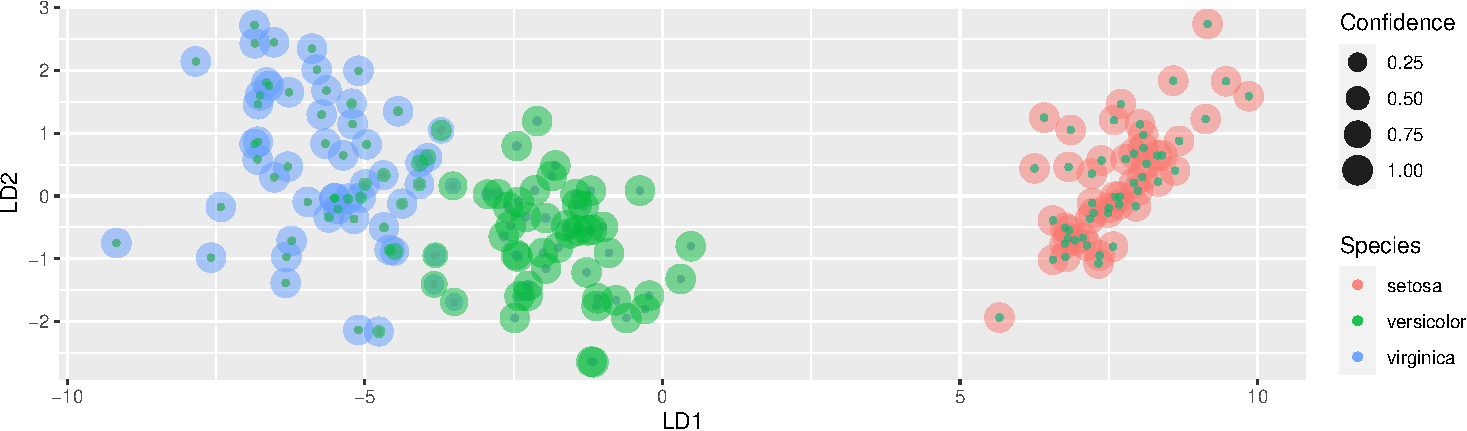
\includegraphics{classify_files/figure-beamer/unnamed-chunk-8-1.pdf}

\end{frame}

\begin{frame}[fragile]{Naive Bayes}
\protect\hypertarget{naive-bayes}{}

With multiple predictors \(x=(x_1, \ldots, x_m)\), assuming that the
distribution \(f_k(x)\) is a product of terms involving only one \(x_i\)
at a time gives a form for \(\delta_k(x)\) that is useful for large
numbers of predictors. (\(m>>0\))

\scriptsize

\begin{Shaded}
\begin{Highlighting}[]
\NormalTok{nb.mod <-}\StringTok{ }\KeywordTok{naiveBayes}\NormalTok{(Species}\OperatorTok{~}\NormalTok{., }\DataTypeTok{data=}\NormalTok{iris)}
\NormalTok{nb.pred <-}\StringTok{ }\KeywordTok{predict}\NormalTok{(nb.mod, }\DataTypeTok{newdata =}\NormalTok{ iris)}
\KeywordTok{sum}\NormalTok{(nb.pred}\OperatorTok{!=}\NormalTok{iris}\OperatorTok{$}\NormalTok{Species)}
\end{Highlighting}
\end{Shaded}

\begin{verbatim}
## [1] 6
\end{verbatim}

\begin{Shaded}
\begin{Highlighting}[]
\KeywordTok{ggplot}\NormalTok{(lda.obs, }\KeywordTok{aes}\NormalTok{(LD1, LD2, }\DataTypeTok{color=}\NormalTok{nb.pred))}\OperatorTok{+}\KeywordTok{geom_point}\NormalTok{()}\OperatorTok{+}
\StringTok{  }\KeywordTok{labs}\NormalTok{(}\DataTypeTok{color=}\StringTok{"Naive Bayes Prediction"}\NormalTok{)}
\end{Highlighting}
\end{Shaded}

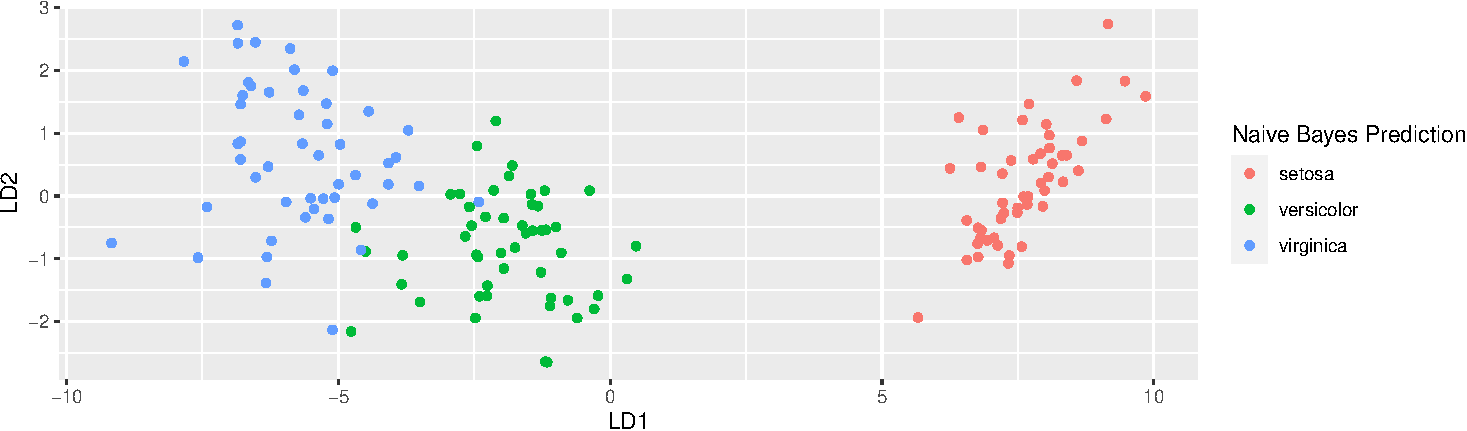
\includegraphics{classify_files/figure-beamer/unnamed-chunk-9-1.pdf}

\end{frame}

\begin{frame}[fragile]{Trees}
\protect\hypertarget{trees}{}

Decision trees are very intuitive.

\scriptsize

\begin{Shaded}
\begin{Highlighting}[]
\NormalTok{tree.iris=}\KeywordTok{prune.tree}\NormalTok{(}\KeywordTok{tree}\NormalTok{(Species}\OperatorTok{~}\NormalTok{.,iris), }\DataTypeTok{best=}\DecValTok{4}\NormalTok{); }\KeywordTok{summary}\NormalTok{(tree.iris)}
\end{Highlighting}
\end{Shaded}

\begin{verbatim}
## 
## Classification tree:
## snip.tree(tree = tree(Species ~ ., iris), nodes = c(7L, 12L))
## Variables actually used in tree construction:
## [1] "Petal.Length" "Petal.Width" 
## Number of terminal nodes:  4 
## Residual mean deviance:  0.1849 = 26.99 / 146 
## Misclassification error rate: 0.02667 = 4 / 150
\end{verbatim}

\begin{Shaded}
\begin{Highlighting}[]
\KeywordTok{plot}\NormalTok{(tree.iris); }\KeywordTok{text}\NormalTok{(tree.iris,}\DataTypeTok{pretty=}\DecValTok{0}\NormalTok{)}
\end{Highlighting}
\end{Shaded}

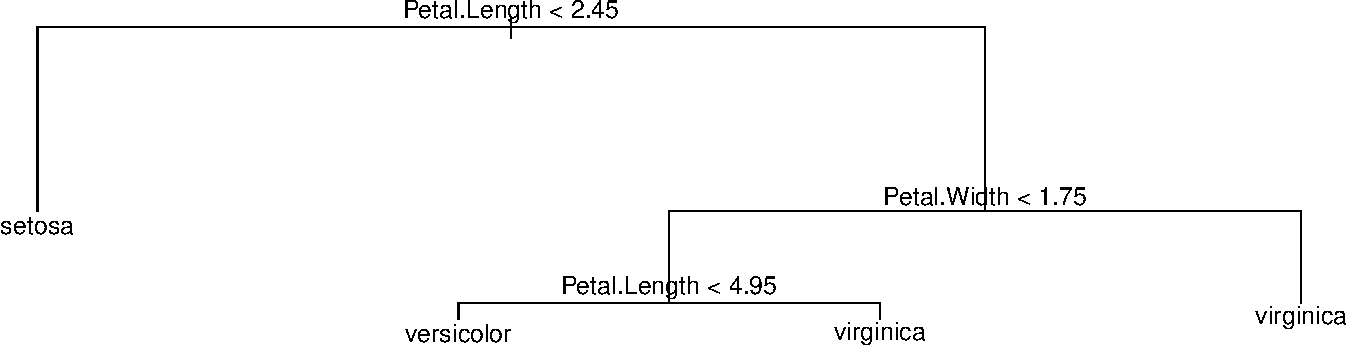
\includegraphics{classify_files/figure-beamer/unnamed-chunk-10-1.pdf}

\end{frame}

\begin{frame}{Tree Building}
\protect\hypertarget{tree-building}{}

Building a tree consists of recursively splitting the data into regions
using thresholds on the predictors.

The process is \emph{top-down} and \emph{greedy}.

\begin{itemize}
\tightlist
\item
  Top-down because we start with unlabeled data and perform the best
  split.
\item
  Greedy because we don't look ahead and make any sub-optimal split that
  will then allow for better splits further down the tree.
\end{itemize}

After building a tree, we need to prune it back to avoid overfitting.
The degree of pruning is a parameter that can be tuned using cross
validation.

\end{frame}

\begin{frame}{Tree Building Details}
\protect\hypertarget{tree-building-details}{}

To determine the best split, we use \emph{Gini index} or
\emph{cross-entropy}. Both are defined for a region (subset of the data
domain) corresponding to a node/leaf of the tree.

\begin{itemize}
\tightlist
\item
  The Gini index: \[
  G=\sum_{k=1}^K\hat p_{k}(1-\hat p_{k})
  \] where \(\hat p_{k}\) is the proportion of training observations in
  the region that are from the \(k\)th class.
\item
  The cross-entropy: \[
  D=-\sum_{k=1}^K\hat p_{k}\log\hat p_{k}
  \]
\end{itemize}

These two measures are similar numerically. Small values indicate that
the region in question is homogeneous.

\end{frame}

\begin{frame}{Unfortunately \ldots}
\protect\hypertarget{unfortunately}{}

Single trees do poorly at predicting compared to the other methods we
have studied.

\end{frame}

\begin{frame}{Random Forests and Bagging}
\protect\hypertarget{random-forests-and-bagging}{}

By building a lot of trees, adding noise to the process as we do so, and
then aggregating the predictions we can build very effective predictive
models.

\begin{itemize}
\tightlist
\item
  \emph{Bagging} (bootstrap aggregation) in a general technique for
  building many models and averaging them. Bootstrap samples of the data
  are used to create replicates of the data for training models.
\item
  The \emph{Random Forest} algorithm builds trees on bootstrapped
  training samples, but at each step, only a random subset of the
  predictors are considered as options for defining a split.
\item
  These additions of noise result in models with lower variance and
  higher predictive power.
\end{itemize}

\end{frame}

\begin{frame}[fragile]{Random Forest Example}
\protect\hypertarget{random-forest-example}{}

\scriptsize

\begin{Shaded}
\begin{Highlighting}[]
\NormalTok{west_fork <-}\StringTok{ }\KeywordTok{read.csv}\NormalTok{(}\StringTok{"data/FieldPlots_WithSpatial.csv"}\NormalTok{)}
\NormalTok{west_fork}\OperatorTok{$}\NormalTok{bc_sqrt_}\DecValTok{7}\NormalTok{ <-}\StringTok{ }\KeywordTok{factor}\NormalTok{(west_fork}\OperatorTok{$}\NormalTok{bc_sqrt_}\DecValTok{7}\NormalTok{)}
\NormalTok{rf.mod <-}\StringTok{ }\KeywordTok{randomForest}\NormalTok{(bc_sqrt_}\DecValTok{7}\OperatorTok{~}\NormalTok{.,}
                       \DataTypeTok{data =}\NormalTok{ west_fork[, }\KeywordTok{c}\NormalTok{(}\DecValTok{4}\NormalTok{,}\DecValTok{8}\OperatorTok{:}\DecValTok{32}\NormalTok{)], }\DataTypeTok{importance=}\OtherTok{TRUE}\NormalTok{)}

\NormalTok{accuracy <-}\StringTok{ }\ControlFlowTok{function}\NormalTok{(tab)}\KeywordTok{sum}\NormalTok{(}\KeywordTok{sapply}\NormalTok{(}\DecValTok{1}\OperatorTok{:}\KeywordTok{nrow}\NormalTok{(tab), }
                                    \ControlFlowTok{function}\NormalTok{(x)tab[x,x]))}\OperatorTok{/}\NormalTok{(}\KeywordTok{sum}\NormalTok{(tab))}
\NormalTok{rf.tab <-}\StringTok{ }\KeywordTok{table}\NormalTok{(}\KeywordTok{predict}\NormalTok{(rf.mod),west_fork}\OperatorTok{$}\NormalTok{bc_sqrt_}\DecValTok{7}\NormalTok{)}
\NormalTok{rf.tab}
\end{Highlighting}
\end{Shaded}

\begin{verbatim}
##    
##      1  2  3  4  5  6  7
##   1  8  0  4  0  0  3  2
##   2  0 89  4 19 10  4  0
##   3 20 10 60  9  0  3 17
##   4  0 10  6 19  2  0  3
##   5  0  2  1  0  4  0  0
##   6  0  0  0  0  0  0  0
##   7  0  0  1  1  0  0  1
\end{verbatim}

\begin{Shaded}
\begin{Highlighting}[]
\KeywordTok{accuracy}\NormalTok{(rf.tab)}
\end{Highlighting}
\end{Shaded}

\begin{verbatim}
## [1] 0.5801282
\end{verbatim}

\end{frame}

\begin{frame}[fragile]{Variable Importance}
\protect\hypertarget{variable-importance}{}

Interpretation of a Random Forest is challenging, but we can get
relative levels of variable importance by looking at decreases in the
Gini index over all the splits where a particular variable is used.

\scriptsize

\begin{Shaded}
\begin{Highlighting}[]
\KeywordTok{varImpPlot}\NormalTok{(rf.mod)}
\end{Highlighting}
\end{Shaded}

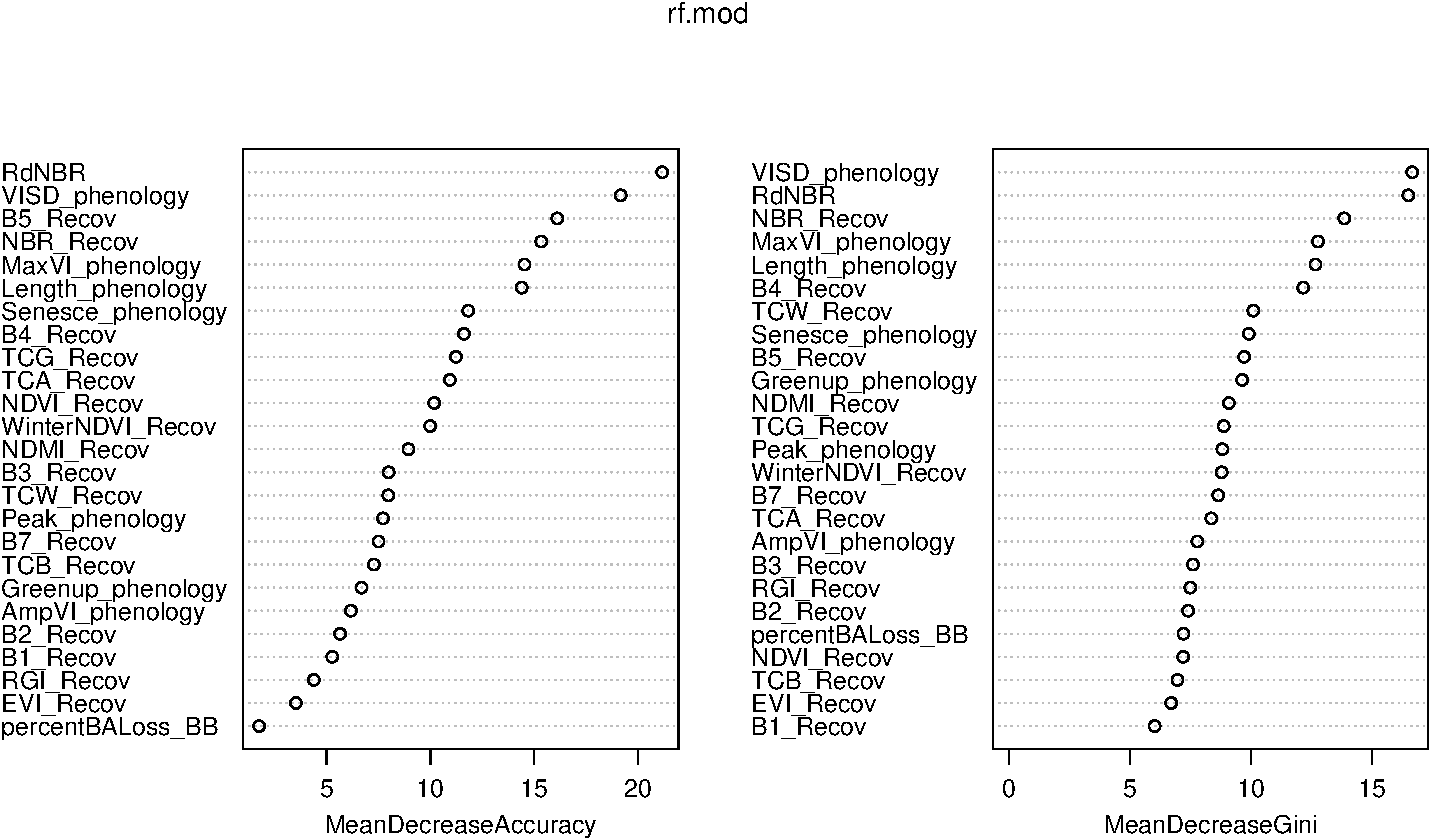
\includegraphics{classify_files/figure-beamer/unnamed-chunk-12-1.pdf}

\end{frame}

\begin{frame}{References}
\protect\hypertarget{references}{}

\hypertarget{refs}{}
\leavevmode\hypertarget{ref-islr}{}%
James, Gareth, Daniela Witten, Trevor Hastie, and Robert Tibshirani.
2013. \emph{An Introduction to Statistical Learning: With Applications
in R}. Springer.
\url{https://faculty.marshall.usc.edu/gareth-james/ISL/}.

\end{frame}

\end{document}
